% !TeX root = ../libro.tex
% !TeX encoding = utf8



\setchapterpreamble[c][0.75\linewidth]{%
	\sffamily
  
    Este capítulo pondrá en conocimiento al lector sobre los aspectos más técnicos que se han llevado a cabo para la elaboración del problema. Primeramente se comenzará hablando del software implementado que se ha empleado y de las cuestiones más importantes del mismo sin entrar mucho en detalle. Posteriormente se comentará el preprocesado realizado en los datos. Tras lo cual, se discutirá sobre la métrica empleada para la evaluación y posterior comparación entre los modelos. Finalmente se esclarecerá el método de selección de los modelos adelantando que será una variación del tradicional método de validación cruzada.
  

	\par\bigskip
}

\chapter{Contexto Experimental}\label{ch:contexto_experimental}


%%%%%%%%%%%%%%%%%%%%%%%%%%%%%%%%%%%%%%%%%%%%%%%%%%%%%%%%%%%%%%%%%%%%%%%%%%%%%%%%%%%%%%%%
%%%%%%%%%%%%%%%%%%%%%%%%%%%%%%%%%%%%%%%%%%%%%%%%%%%%%%%%%%%%%%%%%%%%%%%%%%%%%%%%%%%%%%%%
%%%%%%%%%%%%%%%%%%%%%%%%%%%%%%%%%%%%%%%%%%%%%%%%%%%%%%%%%%%%%%%%%%%%%%%%%%%%%%%%%%%%%%%%

\section{Software}

    El software ha sido implementado en Python, un lenguaje orientado a objetivos muy reconocido por la gran cantidad de herramientas que ofrece. Como librerías se han usado tensorflow junto con keras para la implementación de los modelos además de otras librerías auxiliares: numpy, pandas, seaborn, matplotlib, csv, math, time, sys, os, Sciky-Learn...\\
    
    Para el desarrollo del proyecto ha sido necesario el desarrollo de un conjunto de tres clases cuyos diagramas los podemos encontrar en las figuras \ref{fig:DC1} y \ref{fig:DC2}. Explicamos a continuación la labor que realiza cada una de ellas. La razón de los atributos de instancia así como la funcionalidad de los métodos están comentados en el código por lo que no entraremos en detalle en esa parte, solo mencionaremos las partes más importantes.\\
    
    \begin{itemize}
        \item DataReader: Esta clase está dedicada a la lectura de datos de fichero. El método principal es \textit{\_load\_data} el cual se encarga de leer los datos y no hay que llamarlo, el constructor lo llama directamente una vez se instancia la clase. Únicamente nos tenemos que preocupar de llamar al método \textit{get\_samples\_labels} que es el que nos devuelve los datos leído de fichero, tanto las señales como sus correspondientes etiquetas. 
        \item DataGenerator: Esta clase está dedicada a realizar el aumento de datos. Una vez instanciada podemos generar nuevas señales a partir de las iniciales llamando a los métodos \textit{amp\_signal}, \textit{vertical\_shift}, \textit{horizontal\_shift} y \textit{peaks\_noise}.
        \item CrossValidation: Esta es la clase más importante y se dedica a entrenar el modelo mediante validación cruzada y a sacar los resultados por fichero. Le pasamos al constructor los datos, el modelo junto con una gran cantidad de parámetros. El método principal se llama \textit{cross\_validate} y es al que tenemos que llamar una vez hayamos instanciado la clase. Este método se encarga por dentro de compilar el modelo, entrenarlo mediante validación cruzada y de imprimir los resultados por fichero. Es cierto que se podía haber atomizado más y separarlos en otros métodos. Sin embargo no se ha seguido esta vía ya que se quería hacer un código a muy alto nivel en el que solo se tenga que instanciar el objeto y realizar una única llamada a un método para obtenerlo todo. Esto miso es aplicable a la clase \textit{DataReader}
    \end{itemize}
    
    
    Un fichero llamado \textit{utils.py} ha sido también necesario para definir algunas funciones que nos resultarán de utilidad. El fichero \textit{models.py} contiene los modelos que se han empleado. El resto de ficheros con extensión \textit{.py} son aquellos dedicados a ser ejecutados. Los ficheros con extensión \textit{.sh} son scripts de bash que se han desarrollado con el objetivo de generar una capa de abstracción, de este modo, solo basta ejecutar el scrips y por dentro éste se encarga de iniciar el entorno virtual, buscar un nodo GPU que no esté ocupado, algunas opciones de configuración y de ejecutar el fichero con extensión \textit{.py}. \\
    
    

        \begin{figure}[H]
             \centering
             \begin{subfigure}[b]{0.3\textwidth}
             \includegraphics[scale=0.5]{img/DiagramaClase_DataReader.png}
             \caption{Diagrama de clase de la clase DataReader}
             \label{fig:DC_DataReader}
             \end{subfigure}
             \hfill
             \begin{subfigure}[b]{0.3\textwidth}
             \includegraphics[scale=0.5]{img/DiagramaClase_DataGenerator.png}
             \caption{Diagrama de clase de la clase DataGenerator}
             \label{fig:DC_DataGenerator}
             \end{subfigure}
             \caption{Diagrama de clases de las clases desarrolladas en el proyecto}
             \label{fig:DC1}
         \end{figure}
         \newpage
         \begin{figure}[H]
             \centering
             \includegraphics[scale=0.6]{img/DiagramaClase_CrossValidation.png}
             \caption{Diagrama de clase de la clase CrossValidation}
             \label{fig:DC2}
         \end{figure}
         

%%%%%%%%%%%%%%%%%%%%%%%%%%%%%%%%%%%%%%%%%%%%%%%%%%%%%%%%%%%%%%%%%%%%%%%%%%%%%%%%%%%%%%%%
%%%%%%%%%%%%%%%%%%%%%%%%%%%%%%%%%%%%%%%%%%%%%%%%%%%%%%%%%%%%%%%%%%%%%%%%%%%%%%%%%%%%%%%%
%%%%%%%%%%%%%%%%%%%%%%%%%%%%%%%%%%%%%%%%%%%%%%%%%%%%%%%%%%%%%%%%%%%%%%%%%%%%%%%%%%%%%%%%

\section{Preprocesado}

    La parte del preprocesado de los datos es una de las partes más importantes en ciencia de datos, ya que datos de calidad, aportan resultados de calidad, por lo que no debemos descuidar esta fase. De hecho, la misma plataforma de \textit{physionet} recomiendo tratar los datos antes de aplicar los modelos.\\
    
    \begin{figure}[H]
             \centering
             \begin{subfigure}[b]{0.4\textwidth}
             \includegraphics[scale=0.5]{img/trans_ampl.png}
             \caption{Amplificación}
             \label{fig:data_aug_ampl}
             \end{subfigure}
             \hfill
             \begin{subfigure}[b]{0.4\textwidth}
             \includegraphics[scale=0.5]{img/trans_ruido.png}
             \caption{Picos de Ruido}
             \label{fig:data_aug_ruido}
             \end{subfigure}
             
             \hfill
             
             \begin{subfigure}[b]{0.4\textwidth}
             \includegraphics[scale=0.5]{img/trans_horizontal.png}
             \caption{Desplazamiento horizontal}
             \label{fig:data_aug_horizontal}
             \end{subfigure}
             \hfill
             \begin{subfigure}[b]{0.4\textwidth}
             \includegraphics[scale=0.5]{img/trans_vertical.png}
             \caption{Desplazamiento vertical}
             \label{fig:data_aug_vertical}
             \end{subfigure}
             
             \caption{Transformaciones llevadas a cabo para el aumento de datos. La transformacione se han llevado a cabo sobre la gráfica de una distribución normal de media cero y varianza uno.}
             \label{fig:data_aug}
         \end{figure}
         
    Primeramente se leen los datos en crudo, ocurre que las señales no presentan todas el mismo tamaño, lo que supone un problema para los modelos. Debido a esto se ha de unificar el tamaño de las señales. Para ello se pensaron en muchas alternativas, la primera fue añadir zero-padding a las señales de menor longitud. Este enfoque en la práctica se tradujo en resultados pésimos, ya que las señales más pequeñas, que eran la mayoría, tras añadir el padding, se transformaban en una señal casi constantemente igual a cero. Tras esta perspectiva se decidió fijar un tamaño de ventana y leer de cada señal un subconjunto de la misma de tamaño igual al fijado por la ventana, de este modo evitamos el padding y las señales no son constantemente cero. Había que tener en cuenta que el tamaño de la ventana tenía que ser el suficientemente grande para contener así varios pulsos. Un tamaño de ventana entre 1000 y 5000 es el ideal. \\
    
    
    Tras la lectura de las señales, las normalizamos a media cero y desviación típica uno restando por la media y dividiendo por la desviación típica y teniendo en cuenta los datos que van a parar al conjunto de entrenamiento y al de test para de este modo no cometer \textit{data snooping}. \\ 
    
    Para tratar este desbalanceo se pueden emplear infinidad de técnicas, aunque en el contexto de la competición no son todas válidas. Por ejemplo, se podría pensar en eliminar la clase minoritaria por tener una representación ínfima del conjunto, sin embargo, las reglas establecen que eso no debe hacerse, pues a fin de cuentas, estaremos contaminando los resultados y bajo el supuesto de que el modelo se implemente en la práctica, resultará en algo muy poco fiable y propenso a fallos. De este modo, optamos por la técnica de aumento de datos, para ello nos dedicamos a hacer transformaciones con las señales originales para tener una mayor y variedad. Las distintas transformaciones realizadas las podemos encontrar en la figura \ref{fig:data_aug} donde podemos observar que se hemos realizado desplazamientos horizontales \ref{fig:data_aug_horizontal} y verticales \ref{fig:data_aug_vertical}, amplificaciones de la señal \ref{fig:data_aug_ampl} y picos de ruido \ref{fig:data_aug_ruido}. En la práctica los resultados empeoraban con estas transformaciones y por este motivo se decidió no incluirlas. \\
    
    




%%%%%%%%%%%%%%%%%%%%%%%%%%%%%%%%%%%%%%%%%%%%%%%%%%%%%%%%%%%%%%%%%%%%%%%%%%%%%%%%%%%%%%%%
%%%%%%%%%%%%%%%%%%%%%%%%%%%%%%%%%%%%%%%%%%%%%%%%%%%%%%%%%%%%%%%%%%%%%%%%%%%%%%%%%%%%%%%%
%%%%%%%%%%%%%%%%%%%%%%%%%%%%%%%%%%%%%%%%%%%%%%%%%%%%%%%%%%%%%%%%%%%%%%%%%%%%%%%%%%%%%%%%

\section{Métrica}
    
    Existen una amplia gama de métricas que evalúan el rendimiento de los modelos, en nuestro caso hemos usado la métrica conocida como $F1$. Presentamos primero la matriz de confusión, en la que la posición $(i,j)$ representa el número de ejemplos de la clase $i$ que han sido predichos como elementos de la clase $j$. En la imagen $\ref{fig:metrica}$ también se incluye una columna y una fila adicional que representan la suma de todos los elementos totales de cada clase y la suma del número de prediciones realizadas para esa misma clase. La diagonal de la matriz de confusión aparecen los elementos correctamente clasificados y en la práctica es lo que nos gustaría maximizar. El resto de entradas a excepción de la diagonal y las celdas marginales añadidas, representan instancias mal clasificadas.
    
    \begin{figure}[H]
        \centering
        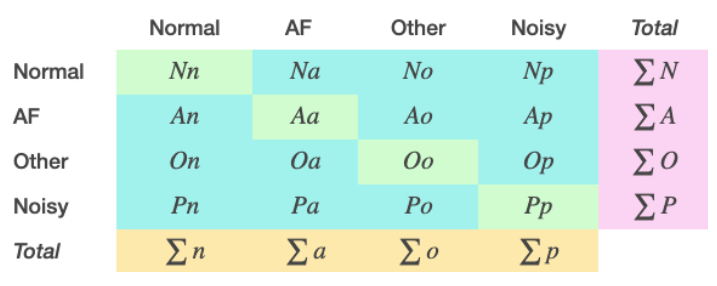
\includegraphics[scale=0.5]{img/metrica.png}
        \caption{Regla para contar el número de variables. En verde se presentan los elementos correctamente clasificados, en azul los incorrectamente clasificados y en naranja y rosa la suma de las columnas y filas respectivamente. \href{https://physionet.org/files/challenge-2017/1.0.0/table3.png}{Fuente}}
        \label{fig:metrica}
    \end{figure}
    
    Para cada una de las clases calculamos su respectiva métrica $F_1$-score de la siguiente manera:
    
    \begin{itemize}
        \item Ritmo normal:
        \begin{equation}
            F_{1n} = \frac{2 Nn}{\sum_{N} + \sum_{n}}
        \end{equation}
        \item Ritmo AF:
        \begin{equation}
            F_{1a} = \frac{2 Aa}{\sum_{N} + \sum_{n}}
        \end{equation}
        \item Otro ritmo:
        \begin{equation}
            F_{1o} = \frac{2 Oo}{\sum_{O} + \sum_{o}}
        \end{equation}
        \item Ruido:
        \begin{equation}
            F_{1p} = \frac{2 Pp}{\sum_{P} + \sum_{p}}
        \end{equation}
    \end{itemize}
    
    \noindent Finalmente, la métrica $F1$ es la media aritmética de estas cuatro,
    \begin{equation}
        F1 = \frac{F_{1n} + F_{1a} + F_{1o} + F_{1p}}{4}
    \end{equation}
    
    El motivo principal existente en cuanto a la elección de esta métrica no es más que subsanar el desbalanceo entre clases otorgando la misma importancia a cada una de ellas. Esto no ocurre en el caso de otras métricas como por ejemplo la \textit{precisión} o \textit{accuracy} la cual expresa el cociente del número de instancias bien clasificadas dividido por el total de instancias. De este modo, en el problema que nos atañe, ocurriría que si un modelo responde correctamente a todos los ejemplos de la clase mayoritaria (Ritmo Normal) y equivocadamente al resto tendría una precisión inferior a $0.6$, lo que nos puede llevar a pensar que el modelo, aunque se equivoque en el $40\%$ de las veces, tiene capacidad de predicción (¡Algo falso!). Del mismo modo y aplicando la métrica $F1$ se obtendría un valor inferior a $0.2$, por lo que de este modo, esta métrica fuerza a construir un modelo en el que la predicción correcta de cada clase influya por igual independientemente del desbalanceo. \\
    
%%%%%%%%%%%%%%%%%%%%%%%%%%%%%%%%%%%%%%%%%%%%%%%%%%%%%%%%%%%%%%%%%%%%%%%%%%%%%%%%%%%%%%%%
%%%%%%%%%%%%%%%%%%%%%%%%%%%%%%%%%%%%%%%%%%%%%%%%%%%%%%%%%%%%%%%%%%%%%%%%%%%%%%%%%%%%%%%%
%%%%%%%%%%%%%%%%%%%%%%%%%%%%%%%%%%%%%%%%%%%%%%%%%%%%%%%%%%%%%%%%%%%%%%%%%%%%%%%%%%%%%%%%

\section{Método de selección de los modelos}

    

    Esta competición cuenta con un conjunto de datos de test a los cuales no hemos tenido acceso por lo que solo hemos empleado los datos de entrenamiento. La selección de los modelos se ha hecho por medio de una variación de la validación cruzada con 5 \textit{folds} la cual se está empezando a emplear mucho en la literatura y consiste en entrenar, validar y aplicar el test en cada fold. \\
    
    Al emplear 5 \textit{folds} realizamos 5 entrenamientos con los datos, en cada entrenamiento dividimos los datos en un conjunto disjunto de entrenamiento, validación y test mediante un muestreo aleatorio estratificado, $S_{train}^i, S_{val}^i$ y $S_{test}^i$ de tal manera que ${S_{train}^i \cap S_{test}^i \cap S_{val}^i = \emptyset}$ y ${S_{train}^i \cup S_{test}^i \cup S_{val}^i = S}$ para $i=\{1,2,3,4,5\}$ . Además, se ha de cumplir que $\bigcap_j S_{test}^j = \emptyset$. Con el muestreo aleatorio estratificado conseguimos que haya la misma proporción de instancias de cada clase en las particiones que el conjunto original. Tras este particionado, se entrena con $S_{train}$, validamos con $S_{val}$ y evaluamos con $S_{test}$.  \\
    
    El motivo de lo anterior es sencillo, obviamente necesitamos el conjunto $S_{train}$ para poder entrenar los datos, el conjunto $S_{val}$ lo usamos para tomar decisiones sobre el entrenamiento, como por ejemplo, la parada del \textit{Early Stopping}, observar la curva de aprendizaje o valorar si se produce o no sobreentrenamiento. Finalmente, $S_{test}$ lo usamos para ver como generaliza y para sacar conclusiones con respecto a otros modelos haciendo así a esta variación de validación cruzada mucho más robusta que la original porque no solo obtenemos la media aritmética de los resultados en cuanto al entrenamiento, sino que también en cuanto a generalización, es decir, en el conjunto de test. \\
    
    Tras la obtención de los resultados en todos los modelos empleados, se elige como modelo ganador aquel con mejores puntuaciones en la métrica $F1$ obtenida con los datos proporcionados por el conjunto de test. \\



\endinput